\chapter{Background Theory and Related Work}

THIS IS AN EXAMPLE. ALL SECTIONS BELOW ARE OPTIONAL. PLEASE CONSULT YOU ADVISOR AND DESIGN YOUR OWN SECTION

\textthai{หัวข้อต่าง ๆ ในแต่ละบทเป็นเพียงตัวอย่างเท่านั้น หัวข้อที่จะใส่ในแต่ละบทขึ้นอยู่กับโปรเจคของนักศึกษาและอาจารย์ที่ปรึกษา}

This is how you add the website URL: \url{http://www.cpe.kmutt.ac.th}

Explain theory, algorithms, protocols, or existing research works and tools related to your work.

You can cite your references like this: \cite{booch87}, or multiplie cite like this: \cite{meyer2000, atwoodmd}

\section{Recommender Systems}

    \begin{table}[!h]
    \caption{test table method1}\label{tbl:method1}
        \begin{tabular}{c|c|l|rr} \hline\hline
            Center & Center & left aligned & Right & Right aligned \\ \hline\hline
            Center & Center & left aligned & Right & Right aligned \\ \hline
            Center & Center & left aligned & Right & Right aligned \\ 
            Center & Center & left aligned & Right & Right aligned \\ \hline
            Center & Center & left aligned & Right & Right aligned \\ \hline\hline
        \end{tabular}
    \end{table}

    You can place any report elements and refer to it like Figure~\ref{tbl:method1}, \ref{fig:oop-concept}
    The figure and table numbering will be run and updated automatically when you add/remove tables/figures from the document.

    \begin{figure}[H]
        \centering
        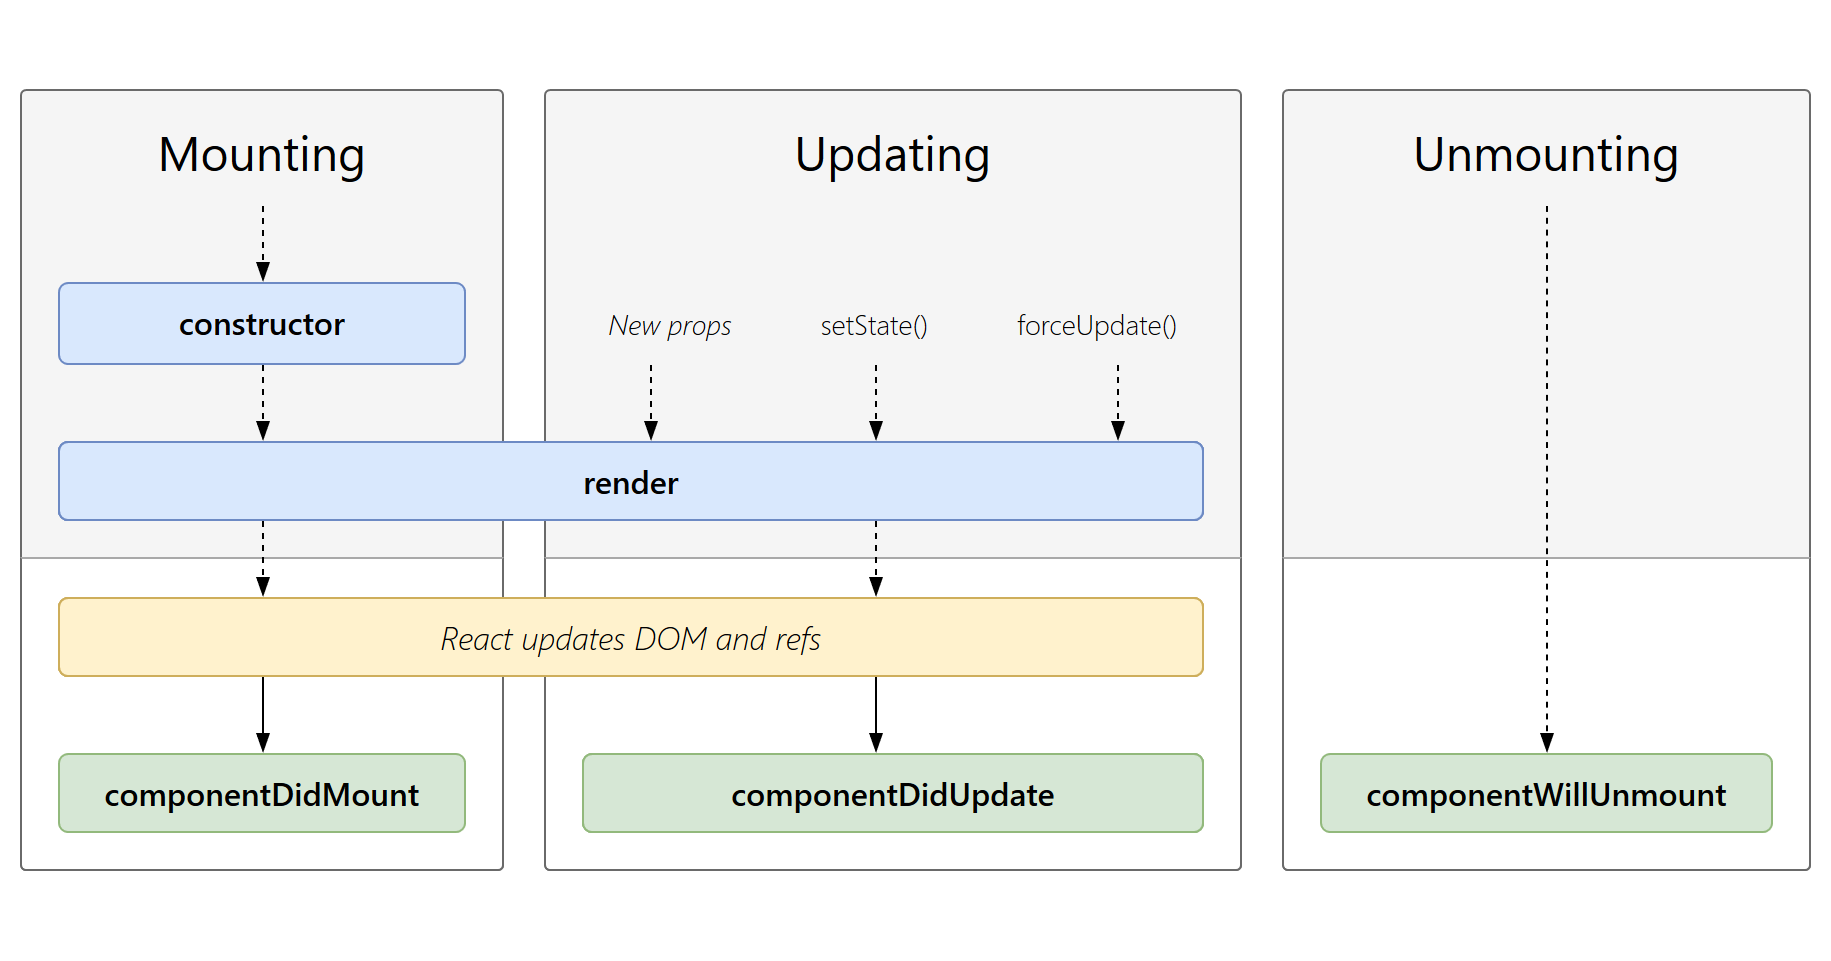
\includegraphics[width=7cm]{chapters/2/figures/react-lifecycle.png}
        \caption[Aspects of OOPs]{Aspects of OOPs from~\cite{apollo22oop}}
        \label{fig:oop-concept}
    \end{figure}
    
    \subsection{Algorithm I}
    Add more subsections as you want.
    \subsection{Algorithm II}
        Add more subsections as you want.
        \subsubsection{Step I}
            You can use subsection too!
        \subsubsection{Step II}
            This is the farthest level of subsection we permitted. (We support only 4th level)


\pagebreak